\documentclass[11pt]{article}
\usepackage{textcomp,bbding,subfig}
\usepackage{float,amssymb,amsmath,amsfonts,bm}
\usepackage{graphicx,cite}
\usepackage[]{natbib}
\def\style{apa}
\usepackage[usenames,pdftex,dvips]{color,xcolor}
\usepackage{multirow,tabulary,colortbl,array}
\usepackage[normalem]{ulem}
\usepackage[colorlinks,bookmarksopen,bookmarksnumbered,citecolor=blue,urlcolor=blue]{hyperref}
\usepackage{moreverb,setspace}

% Text layout
\topmargin -1.5cm
\oddsidemargin 0.0cm
\evensidemargin 0.0cm
\textwidth 16.5cm
\textheight 23.5cm     

% Remove brackets from numbering in List of References
% \makeatletter \renewcommand\@biblabel[1]{} \makeatother
\makeatletter
\renewcommand{\@biblabel}[1]{\quad#1.}
\makeatother
%
% aliasis
% FreeSurfer from Havord Unv.
\newcommand{\FS}{\href{http://surfer.nmr.mgh.harvard.edu}{\textbf{FreeSurfer}}} 
\newcommand{\bs}{\boldsymbol}
%
% vectors and matrices
\newcommand{\vb}{\boldsymbol{b}}
\newcommand{\vc}{\boldsymbol{c}}
\newcommand{\vh}{\boldsymbol{h}}
\newcommand{\vv}{\boldsymbol{v}}
\newcommand{\vx}{\boldsymbol{x}}
%
\newcommand{\mD}{\boldsymbol{D}}
\newcommand{\mV}{\boldsymbol{V}}
\newcommand{\mW}{\boldsymbol{W}}
%
% with hats or tildes
\newcommand{\vbt}{\tilde{\vb}}
\newcommand{\vct}{\tilde{\vc}}
\newcommand{\vht}{\tilde{\vh}}
\newcommand{\vvt}{\tilde{\vv}}
\newcommand{\vvp}{\vv^{\prime}}
\newcommand{\mWt}{\tilde{\mW}}
\newcommand{\vxt}{\tilde{\vx}}
%
% xiaoran's edit
\newcommand{\xadd}[1]{\textcolor{blue}{#1}}
\newcommand{\xdel}[1]{\textcolor{red}{\sout{#1}}}
\newcommand{\xrpl}[2]{\xdel{#1}\xadd{#2}}
\newcommand{\xacc}[1]{\textcolor{ForestGreen}{#1}}
%
% encoders
% vector or matrix
\newcommand{\vecEC}[1]{\boldsymbol{#1}}
%
% decoders
\newcommand{\vecDC}[1]{\boldsymbol{\tilde{#1}}} 
%
\newcommand{\xVO}{\boldsymbol{x}}         % the x vector, original
\newcommand{\xVR}{\boldsymbol{\tilde{x}}} % the x vector, recovered
\newcommand{\xSO}{x}                      % the x scaler, original
\newcommand{\xSR}{\tilde{x}}              % the x scaler, recovered
%
% the eta vector
\newcommand{\etaEC}{\vecEC{\eta}}                % generic encoder
\newcommand{\etaEi}{\WEC_i^{d_{i+1} \times d_i}} % encoder layer i
\newcommand{\etaDC}{\vecDC{\eta}}                % generic decoder
\newcommand{\etaDi}{\WDC_i^{d_i \times d_{i+1}}} % decoder layer i
%
% the W matrix
\newcommand{\WEC}{\vecEC{W}}                   % generic encoder
\newcommand{\WEi}{\WEC_i^{d_{i+1} \times d_i}} % encoder layer i
\newcommand{\WEI}[3]{\WEC_{#1}^{d_{#2} \times d_{#3}}} % decoder layer #i
\newcommand{\WEIt}[3]{\WEC_{#1}^{d_{#2} \times d_{#3}\prime}} % decoder layer #i, transposed
\newcommand{\WDC}{\vecDC{W}}                   % generic decoder
\newcommand{\WDi}{\WDC_i^{d_i \times d_{i+1}}} % decoder layer #i
\newcommand{\WDI}[3]{\WDC_{#1}^{d_{#2} \times d_{#3}}} % decoder layer #i
\newcommand{\WDIt}[3]{\WDC_{#1}^{d_{#2} \times d_{#3}\prime}} % decoder layer #i

% the w vector
\newcommand{\wEC}{\vecEC{w}}    % generic encoder
\newcommand{\wEI}[2]{{\wEC_{#1}^{1 \times d_{#2}}}}
\newcommand{\wDC}{\vecDC{w}}    % generic decoder
\newcommand{\wDI}[2]{{\wDC_{#1}^{1 \times d_{#2}}}}
\newcommand{\wDIt}[2]{{\wDC_{#1}^{1 \times d_{#2}\prime}}}

% the b vector
\newcommand{\bEC}{\vecEC{b}}    % generic encoder
\newcommand{\bEi}{\bEC_i^{d_i}} % encoder layer i
\newcommand{\bEI}[2]{\bEC_{#1}^{d_{#2}}} % encoder layer i
\newcommand{\bDC}{\vecDC{b}}    % generic decoder
\newcommand{\bDi}{\bDC_i^{d_i}} % encoder layer i
\newcommand{\bDI}[2]{\bDC_{#1}^{d_{#2}}} % encoder layer i

% the x vector
\newcommand{\xEC}{\vecEC{x}}
\newcommand{\xDC}{\vecDC{x}}
% the X matrix
\newcommand{\XEC}{\vecEC{X}}
\newcommand{\XDC}{\vecDC{X}}
%
% the y_hat vector
\newcommand{\yHT}{\boldsymbol{\hat{y}}}
\newcommand{\YHT}{\boldsymbol{\hat{Y}}}
\newcommand{\hHT}{\boldsymbol{\hat{h}}}
\newcommand{\HHT}{\boldsymbol{\hat{H}}}
%
% the z vector
\newcommand{\zEC}{\vecEC{z}}
\newcommand{\zDC}{\vecDC{z}}
%
% I/O for decoder layer
\newcommand{\iDi}{\zDC_{i+1}^{d_{i+1}}}
\newcommand{\zEI}[2]{\zEC_{#1}^{d_{#2}}}
\newcommand{\zEIt}[2]{\zEC_{#1}^{d_{#2}\prime}}
\newcommand{\oDi}{\zDC_i^{d_i}}
\newcommand{\zDI}[2]{\zDC_{#1}^{d_{#2}}}
\newcommand{\zDIt}[2]{\zDC_{#1}^{d_{#2}\prime}}
%
% the vector of ones
\newcommand{\one}{\boldsymbol{1}}
% the diagnal matrix
\newcommand{\I}[1]{\boldsymbol{I}^{#1}}
%
% parameters in the neural network
\newcommand{\Par}{\boldsymbol{\Theta}}
\newcommand{\pEC}{\boldsymbol{\theta}}
\newcommand{\pDC}{\boldsymbol{\tilde{\theta}}}
%
% Loss function in Cross Entropy form
\newcommand{\LCE}[2]{#1\log{#2} + (1-#1)\log{(1-#2)}}
%
% derivative
\newcommand{\DRV}[2]{\frac{d #1}{d #2}}
\newcommand{\DRC}[3]{\DRV{#1}{#2}\DRV{#2}{#3}}
\newcommand{\PDV}[2]{\frac{\partial #1}{\partial #2}}
\newcommand{\PDC}[3]{\PDV{#1}{#2}\PDV{#2}{#3}}
%
% invers logit, aka. sigmoid function
\newcommand{\SGM}[1]{\frac{1}{1+e^{-#1}}}
%
% assign to diagnoral
\newcommand{\diag}[1]{\text{diag} (#1)}

% \pagestyle{headings}

% \author{Xiaoran Tong, Qin Lu} 
\doublespacing
\begin{document}
\title{An Joint Association Analysis Method for Genomic Sequencing and Neuroimaging Data}
\maketitle
\begin{flushleft}
Xiaoran Tong\textsuperscript{1},
Qin Lu\textsuperscript{1*},
\\
\bigskip
\textbf{1} Department of Epidemiology and Biostatistics, Michigan State University, East Lansing, USA

\vskip 50ex
Correspondence: Qing Lu\\
Department of Epidemiology and Biostatistics\\
College of Human Medicine\\
Michigan State University\\
909 Fee Road\\
East Lansing, MI 48824-1030\\
qlu@msu.edu\\
\end{flushleft}

\clearpage
\begin{abstract}
The next generation sequencing (NGS) and medical imaging technology give rise to large, multi-site cohort with a growing wealth of NGS and imaging data, which mandates the development of analytic methods capable of utilizing these imaging data to help identify predictive genomic bio-markers to narrow the gap of ``missing heritability'' for complex diseases. The added imaging information also brought challenges old and new, from the high dimensionality - high redundancy of medical data, to the ``curse'' of multiple testing that kills statistical power of any association analysis involving high dimensional data. In this study, we incorporate the imaging profile to empower the genomic association analysis through the use of the similarity U statistic. To tackle the high dimensionality and high redundancy of the imaging profile, we train stacked autoencoders with recent machine learning techniques, and use them to replace the raw imaging with abstracted high order features. To counter the lack of power due to multiple testing, we apply the signal aggregation practice seen in genomic association studies to the new imaging data.
The simulation and real data analysis are conducted using the NGS and neuroimaging data provided by the Alzheimer’s Disease Neuroimaging Initiative (ADNI). We demonstrate that the joint analysis outperfroming the use of either genome or neuroimaging profile alone, the improvement achieved by replace raw neuroimaging with high order features, and the benefit of grouping and aggregation on neuroimaging data.
\end{abstract}
\clearpage

\section*{Introduction}

\section*{Methods}

\subsection*{Restricted Boltzmann Machine}
The Restricted Boltzmann Machine (RBM) is an engergy based model that treats the observed data as the visible portion of the states existing in a physics system. Besides the $P$ visible units from the observation, denoted by vector $\vv$, a state in such a system also contains $Q$ unobserved hidden unites denoted by $\vh$. The visible and hidden units are fully connected, but are not connected within themselves, as shown in Figure \ref{fig:rbm}.
\begin{figure}[!htbp]
  \centering
  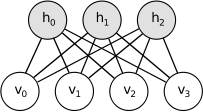
\includegraphics[width=100px]{img/rbm.png}
  \caption{The Restricted Boltzmann Machine.}\label{fig:rbm}
\end{figure}
Together $\vv$ and $\vh$ comprise a system state $(\vv, \vh)$, and by analogy of a physics system, every configuration of $(\vv, \vh)$ has its own energy, which is the exponential of the negative potential $-E(\vv, \vh)$:
\begin{equation*}
  energy(\vv, \vh) = e^{-E(\vv, \vh)}.
\end{equation*}
The exact function form of potential $E(\vv, \vh)$ is designed to suit specifit characteristic of the sytem and to ease the computation, which will be discussed later. Now to continue the analyog of physics that says the states of lower energy are more prevalent, while rarer states require higher energy, we assign probability to each distinctive state $(\vv, \vh)$ according to its energy $e^{-E(\vv, \vh)}$:
\begin{equation} \label{eq:prob0}
  \begin{split}
    \Pr(\vv, \vh) = \frac{e^{-E(\vv, \vh)}}{Z}, \quad Z = \int_{\vv,\vh}{e^{-E(\vv, \vh)}d(\vv, \vh)},
  \end{split}
\end{equation}
thus high engery requirement deter a state from occurring while low engery does encourages it. The partition function $Z$ is the integral of energy over distinct states, which is the normalizing constant of the Boltzmann distribution with density $\Pr(\vv, \vh)$. In such a system, the likelihood of obtaining a sample $\vvt$, that is, one of the assignment of visible units, is the marginal probability of $\Pr(\vvt, \vh)$ over $\vh$, that is,
\begin{equation} \label{eq:probv}
  \begin{split}
    \Pr(\vvt) = \int_{\vh}{\Pr(\vvt, \vh)d\vh} = \frac{1}{Z} \int_{\vh}{e^{-E(\vvt, \vh)}d\vh}
  \end{split}
\end{equation} 
The modeling objective is to find the system that miximizes the overall likelihood of seeing $N$ samples of the data, $\mD=[\vv_1^\prime, \vv_2^\prime, \dots, \vv_N^\prime]$, which in the log scale is
\begin{equation} \label{eq:objective}
  \begin{split}
    l(\mD) &= \sum_{k=1}^N{\log{\Pr(\vv_k)}} \\
    &= \sum_{k=1}^N{[\log{\int_{\vh}{e^{-E(\vv, \vh)}d\vh}} - \log{Z}]}
  \end{split}
\end{equation}
For now we limit our discussion on binary systems, that is, $v$ and $h$ take values from \{0, 1\}, the potential function $E(v, h)$ uses the following form:
\begin{equation} \label{eq:energy}
  E(\vv, \vh) = -\bs{b}^\prime \vv - \bs{c}^\prime \vh - \vh^\prime \bs{W} \vv,
\end{equation}
where the entries in P-vector $\bs{b}$ dictates the negative energy contributed to the system when the cooresponding visible units in $\vv$ are turned on (i.e., taking value 1), thus larger $b_i, (i=1, \dots, P)$ means more energy drained when $v_.i$ is on, making states with $v_i=1$ relatively more predominant. The Q-vector $\bs{c}$'s entries are interpreted in the same manner, that is, larger $c_.j, (j=1, \dots, Q)$ promotes states with active $h_{.j}$. The entries in the weight matrix $\bs{W}$ determines the connection between pairs of visible and hidden unit, visualized as the edges in Figure \ref{fig:rbm}. A large $W_{ij}$ either encourages (when positive) or prohibits (when negative) co-activation of $v_{.i}$ and $h_{.j}$, while a small $W_{ij}$ diminish inter-dependency of the two units. 


\subsection*{Processing Genomic Profile with Stacked Autoencoder}
\xacc{Rooted in Artificial Intellegence (AI), a Stacked Autoencoder (SA) is a type of artificial neural network mimicking visual processing that abstracts high order features from a raw image, which are far more relevant to the decision making of a sentient being than the exact pixel values in the original image. As a physician, knowing the exact thickness and curvature of every point in the 3D cortex image does not help the diagnosis of neurodegenerative disorders, instead, being able to recognize general location, size and shape of the laceration sites in the same cortex image significantly boost the sensitivity and specificity of his judgement. Thus, by learning high order features with the SA while disregarding trivial and redundant details, we expect to achieve a power boost in a subsequent association analysis, given that these features are appropriate for replacing the unprocessed imaging profile.}

A stacked autoencoder is comprised of two or more encoders stacked on top of each other. An encoder is an information preserving transformation that produces output more concise than the input, which, in our case, is the linear recombination of the input entries followed by an entry-wise non-linear transformation. For a stack of $M$ layers of encoder, the $i$th encoder can be written as:
\begin{equation} \label{eq:AE}
  \zEC_i^{d_i} = \boldsymbol{s}(\WEI{i}{i}{i-1} \zEI{i-1}{i-1} + \bEI{i}{i}), \quad i = 1, \ldots, M
\end{equation}
where $\zEI{i}{i}$ is the $i$th encoder's $d_i$ dimensional output, and $\zEI{i-1}{i-1}$ is $d_{i-1}$ dimensional input, which, in turn, is also an output from the encoder down below, (i.e., $(i-1)$th in the stack). The linear recombination of input is done by the $d_{i-1} \times d_i$ weight matrix $\WEI{i}{i}{i-i}$ and the size $d_i$ offset vector $\bEI{i}{i}$. The symbol $\boldsymbol{s}(\cdot)$ denotes the aforementioned entry-wise non-linear transformation, a popular choice for is the ``$S$" shaped inverse logit function (a.k.a sigmoid function) that mimics neuron activation~\cite{SGM1, NNE90}. Finally, being an encoder demands the output size $d_i$ smaller than the input size $d_{i-1}$, which in turn ensures that dimension reduction and high order feature abastraction actually happen. We let the encoders halve its input. \textcolor{red}{Do you need to have it here, given the next paragraph?}

\xacc{Once an encoder is defined,} one can assemble a stack of $M$ encoders that accepts size $P$ input vector, $\xEC^P$, and produces size $Q<P$ high order feature vector, $\hHT^Q$, by recursively wiring the output of an encoder is to the one above it, and ensuring that the input dimensionality at the bottom, $d_0$, equals to $P$, and the output dimensionality on the top, $d_M$, equals to $Q$. Mathematically, the encoder stack can be written as:
\begin{equation} \label{eq:SE}
  \begin{split}
    \hHT^Q &= \zEI{M}{M} \\
    \zEI{M  }{M  } &= s(\WEI{M  }{M  }{M-1} \zEI{M-1}{M-1} + \bEI{M  }{M  }) \\
    \zEI{M-1}{M-1} &= s(\WEI{M-1}{M-1}{M-2} \zEI{M-2}{M-2} + \bEI{M-1}{M-1}) \\
    & \quad \quad \quad \quad \vdots \\
    \zEI{i  }{i  } &= s(\WEI{i  }{i  }{i-1} \zEI{i-1}{i-1} + \bEI{i  }{i  }) \\
    & \quad \quad \quad \quad \vdots \\
    \zEI{2  }{2  } &= s(\WEI{2  }{2  }{1  } \zEI{1  }{1  } + \bEI{2  }{2  }) \\
    \zEI{1  }{1  } &= s(\WEI{1  }{1  }{0  } \zEI{0  }{0  } + \bEI{1  }{1  }) \\
    \zEI{0  }{0  } &= \xEC^P.
  \end{split}
\end{equation}
Here, the $P$-dimensional input $\xEC^P$ can be viewed as the output of the non-existing $0$th encoder. By ensuring that $P = d_0 > d_1 > d_2 > \dots > d_{M-1} > d_M = Q$, the encoder stack abstracts $Q$ dimensional high order features from the $P$ dimensional raw profile. Now, to ensure the output actually being a concise preservation of the input, the parameters of the stack, that is, the weights and the offsets, $\{\WEC_1, \bEC_1, \WEC_2, \bEC_2, \dots, \WEC_M, \bEC_M\}$, must be tuned to represent the body of knowledge that generated $\xEC^P$, which in our case is the knowledge of human cortex. To do so, we assemble a stacked encoder counterpart, i.e., a stacked decoder that starts with higher order features and outputs the entire image. The stacked decoders exactly mirror the topology of the initial encoders:
\begin{equation} \label{eq:SD}
  \begin{split}
    \xDC^P &= \zDI{0}{0} \\
    \zDI{0  }{0  } &= s(\WDI{1  }{0  }{1  } \zDI{1  }{1  } + \bDI{1  }{0  }) \\
    \zDI{1  }{1  } &= s(\WDI{2  }{1  }{2  } \zDI{2  }{2  } + \bDI{2  }{1  }) \\
    & \quad \quad \quad \quad \vdots \\
    \zDI{i-1}{i-1} &= s(\WDI{i  }{i-1}{i  } \zDI{i  }{i  } + \bDI{i  }{i-1}) \\
    & \quad \quad \quad \quad \vdots \\
    \zDI{M-2}{M-2} &= s(\WDI{M-1}{M-2}{M-1} \zDI{M-1}{M-1} + \bDI{M-1}{M-2}) \\
    \zDI{M-1}{M-1} &= s(\WDI{M  }{M-1}{M  } \zDI{M  }{M  } + \bDI{M  }{M-1}). \\
  \end{split}
\end{equation}
The weights of the stacked decoders also mirror the weights of the stacked encoders:
\begin{align}
  \WDI{M-i}{M-i-1}{M-i} \equiv {(\WEI{M-i}{M-i}{M-i-1})}^\prime, \quad (i=0, \dots, M),
\end{align}
However, the offsets in the decoders, $\bDI{M-i}{M-i-1}, (i=0, \dots, M)$, are allowed to be flexible \citep{DL:SDA1}. This approach to tuning the parameters of the stack is quiet instinctive since decoding is the opposite of encoding. From the bottom to the top, this stack of decoders gradually restores details back to the abstracted state $\zDI{M}{M}$ and eventually presents a reconstructed input $\xDC^P$ on its top.

One can combine Equations (\ref{eq:SE}) and (\ref{eq:SD}) by setting $\zDI{M}{M} = \hHT^Q$,
\begin{equation} \label{eq:SA}
  \begin{split}
    \xDC^P &= \zDI{0}{0} \\
    \zDI{0  }{0  } &= s(\WDI{1  }{0  }{1  } \zDI{1  }{1  } + \bDI{1}{0  }) \\
    & \quad \quad \quad \quad \vdots \\
    \zDI{M-1}{M-1} &= s(\WDI{M  }{M-1}{M  } \zDI{M  }{M  } + \bDI{M}{M-1}) \\
    \zDI{M  }{M  } &= \hHT^Q = \zEI{M}{M} \\
    \zEI{M  }{M  } &= s(\WEI{M  }{M  }{M-1} \zEI{M-1}{M-1} + \bEI{M}{M  }) \\
    & \quad \quad \quad \quad \vdots \\
    \zEI{1  }{1  } &= s(\WEI{1  }{1  }{0  } \zEI{0  }{0  } + \bEI{1}{1  }) \\
    \zEI{0  }{0  } &= \xEC^P,
  \end{split}
\end{equation}
which creates a stacked autoencoder \citep{DL:SDA1}. The aforementioned weights and offsets in the encoder stack (the lower half of the SA), alongside with $M$ extra offsets in the decoder stack (the upper half of the SA), constitute the parameters to be calibrated in order to make the encoder stack to be a close represent of the process that generated $\xEC^P$. The calibration is done by minimize the discrepancy between the reconstructed input $\xDC^P$ and the true input $\xEC^P$. The rationale is that if the compact code $\hHT$ presented by the encoder stack truly captures the major features of $\xEC^P$, the restored input, $\xDC^P$, should be nearly identical to the original one, except some trivial details. Tuning the encoder stack is equivalent to solving the following optimization problem:
\begin{equation} \label{eq:CE}
  \begin{split}
    \Par^* = \min_{\Par} \sum_{k=1}^N{d(\xDC_k^P, \xEC_k^P)}, \quad \Par = \cup_{i=1}^M \{\WEC_i, \bEC_i, \bDC_i\},
  \end{split}
\end{equation}
where $k$ indices $N$ training samples. The objective function, $d$, measures the disagreement between the reconstructed and the original input. A popular form of $d$ is a cross-entropy:
\begin{align} \label{eq:CE}
  d(\xDC_k^P, \xEC_k^P) = \sum_{j=1}^P[{x_{j,k}\log{\tilde{x}_{j,k}} + (1 - x_{j,k})\log{(1 - \tilde{x}_{j,k})}}],
\end{align}
where $j$ indices $P$ entries of the input. 

Optimization of a large number of parameters (\xdel{cardinality of }$|\Par| = \sum_{i=1}^M{d_i d_{i-1} + d_i + d_{i-1}}$) is achieved by stochastic gradient descent (SGD)~\citep{SGD1, SGD2}, which is also called the back propagation (BP) algorithm by neural network literature concerning computations of high dimensional gradients ~\citep{BP1, BP2, BP3}. For practical implementation of SGD and BP algorithms, a Python~\citep{python1} library Theano~\citep{Theano1} can be used.

Optimization of deep neural networks, (i.e., a SA of many layers of encoder and decoder) is challenged by increased local minimum site in the error terrian and decreased convergence rate. The counter this issue, we follow the recently popular ``deep learning'' trend, by which a layer-wise greedy pre-training procedure is applied prior to fine-tuning the entire network~\citep{DL:DBN1, DL:SDA1}. To do so, the output of the $i$th encoder, $\zEC_i$, is disconnected from the encoder above it and rewired to its decoder's counterpart, immediately forming a single layered autoencoder, which is then calibrated by minimizing the intermediate reconstruction loss $d(\zEC_{i-1}, \zDC_{i-1})$. That is,
\begin{equation}\label{eq:Greedy}
  \begin{split}
    \zDC_{i-1} &= s(\WDC_i \zDC_i + \bDC_i) \\
    \zDC_{i  } &= \hHT_i = \zEC_i \quad \qquad \qquad \qquad (i = 0 \dots M) \\
    \zEC_{i  } &= s(\WEC_i\zEC_{i-1} + \bEC_i). \\
    \pEC_i^* &= \min_{\pEC_i}{d(\zEC_{i-1}, \zDC_{i-1})}, \qquad \pEC_i = \{\WEC_i, \bEC_i, \bDC_i\},
  \end{split}
\end{equation}
This optimization problem is a much easier than the one in Eq. (\ref{eq:SA}) due to a smaller number of parameters ($|\pEC_i|=d_i d_{i-1} + d_i + d_{i-1}$). After all $M$ single-layer autoencoders are pre-trained, the encoders and decoders are wired back to Eq. (\ref{eq:SE}) (\textcolor{red}{are you sure this is the right equation?}) and fine-tuned together, resulting in faster convergence and less likely chances of ``going down the wrong pit'' in the terrian of $d(\xDC_k^P, \xEC_k^P)$.

% \subsection*{Joint Test with Similarity U}
% \newcommand{\vg}{\boldsymbol{g}}
% \newcommand{\vv}{\boldsymbol{v}}
% We use a similarity U statistic~\cite{UST1, UST2} to jointly test the existence of association among genomic, imaging and phenotype profiles. To derive the statistic, three kernel functions measuring pairwise similarity are chosen for each profile. The measurement $f$ can be flexible to suit the charisteristics of the profile (e.g.\ bounded or not, continuous or discrete), as long as $f$ is symmetric and finite in the second moment, that is, $f(x_i,x_j) \equiv f(x_j,x_i)$ and $E(f^2(x_i, x_j))<+\infty$.

% For genomic profile coded by minor allele count 0, 1 or 2, we use the Identical By State (IBS) kernel
% \label{eq:wSG}
% \[ f_G(\vg_{i.}, \vg_{j.}) = \frac{\sum_{m=1}^{|G|}{w_m(2 - |g_{im} - g_{jm}|)}} {2\sum_{m=1}^{|vG|}{w_m}}, \]
% where $(i,j)$ indices a pair of observations, and $m$ indices a genomic variant (i.e.\ a SNP) in the testing unit (i.e.\ a gene); $w_m$ is the weight assigned to the $m$ th.\ variant according to \textit{a prior} hypothesis, such as allele frequency (AF) based $w_m=\sqrt{AF(g_{.m})[1-AF(g_{.m})]}$ that emphasizes the effect of rare variants.

% The imaging profile can either be the raw 3D cortical surface vertices or the high order features abstracted from them by an SA, for both we can use the Gaussian kernel which is better suited for continuous value,
% \label{eq:wSV}
% \[ f_V(v_{i.},v_{j.}) = \exp{ [-\frac{\sum_{m=1}^{|V|}{w_m{(u_{im}-u_{jm})}^2}} {\sum_{m=1}^{|V|}{w_m}}] }. \]
% Here $m$ indices a imaging variant (i.e.\ a vertex), other notations means the same.

% Lastly, for a phenotype profile generated by unknown distribution, it is first normalized with the rank normal quantile transformation
% \[ q = \frac{\Phi^{-1}[rank(y - 0.5)]}{N}, \]
% where $N$ is the number of observations. The phenotype similarity is also measured by a Gaussian kernel, simplied because the phenotype is one dimensional,
% \[ f_Y(q_i, q_j) = \exp{[-{(q_i - q_j)}^2]}. \]

% The similarity measure for a pair $(i, j)$ is centralized by substracting the two marginal mean measure involving either $i$ or $j$, then adding the grand mean~\cite{UST1}:
% \begin{align*}
%   \tilde{f}(*_i, *_j) = f(*_i, *_j)-\frac{1}{N} \sum_{k=1}^N{f(*_i, *_k)}-\frac{1}{N}\sum_{l=1}^N{f(*_l, *_j)} + \frac{1}{N^2} \sum_{k=1}^{N} \sum_{l=1}^{N} {f(*_l, *_k)}.
% \end{align*}
% Finally, the joint similarity U statistics $U_J$ is the mean of entry-wise product of centralized measurements excluding the self-pairs, which is
% \[ U_J = \frac{2}{N(N-1)} \sum_{1 \leq i < j \leq N}^{} \tilde{f}_G(\vg_{i.}, \vg_{j.}) \circ \tilde{f}_V(\vv_{i.}, \vv_{j.}) \circ \tilde{f}_Y(y_i, y_j), \]
% where $\circ$ means entry-wise product. When there is no association among any of the profiles, $U_J$ should be close to $0$ since all the measurements have mean $0$. Conversely, if $U_J$ deviates from $0$ significantly, it means the similarity regarding one profile is correlated to that regarding other profiles, implying the presence of association. Formally, under $H_0^J$: there is no association between any of the profiles, $U_J$ follows a $\chi_1^2$ mixture weighted by the squared engien values of $\tilde{f}_G(\vg_{i.}, \vg_{j.}) \circ \tilde{f}_V(\vv_{i.}, \vv_{j.}) \circ \tilde{f}_Y(y_i, y_j)$~\cite{UST1, UST2}. The p-value is calculated using Davis method~\cite{davies80}.

% Alternatively, two simpler tests can be done by dropping either the imaging or genomic kernal. Thus,
% \[ U_G = \frac{2}{N(N-1)} \sum_{1 \leq i < j \leq N}^{} \tilde{f}_G(\vg_{i.}, \vg_{j.}) \circ \tilde{f}_Y(y_i, y_j) \]
% tests $H_0^G$: there is no association between the phenotype and genomic profiles. And,
% \[ U_V = \frac{2}{N(N-1)} \sum_{1 \leq i < j \leq N}^{} \tilde{f}_V(\vv_{i.}, \vv_{j.}) \circ \tilde{f}_Y(y_i, y_j) \]
% tests $H_0^V$: there is no association between the phenotype and imaging profiles. These two tests are more specific thus may produce more parsimonious models, but also risk mis-specification, which is to be examed by simulation study.

% The imaging similarity by design is an aggregation of signals of all vertices in the testing unit. For comparison purpose, we also implement the vertex-wise analysis (VWA). Briefly speaking, we first smooth the imaging profile with a Gaussian filter of standard deviation 2, which reduces the noise by grinding away trivial details in the 3D cortex. Next, we treat the orginal $|V|$ dimensional testing unit as $|V|$ one dimensional profiles, and perform that many times of $U_J$ or $U_V$ tests. The resulting $|V|$ p-values are corrected by FDR (false discovery rate) against multiple testing. If any of the corrected p-values is below the $0.05$ threshold, the entire testing unit of $|V|$ vertices is declared statistically significant.

%
% \input{tex/sec_intro}
% \input{tex/sec_method}
% \input{tex/sec_result}
% \input{tex/sec_dissc}
%
\singlespacing 
\bibliographystyle{\style}
\bibliography{ref}

\end{document}

%%% Local Variables:
%%% mode: latex
%%% TeX-master: t
%%% End:
